\immediate\write18{makeindex -s nomencl.ist -o "\jobname.nls" "\jobname.nlo"}
%
% TODO:
%     - seeds for algo 2
%     - discuss results
%     - spline path
%     -
%
%
\documentclass[conference]{IEEEtran}

% *** CITATION PACKAGES ***
%
\usepackage{cite}

% *** GRAPHICS RELATED PACKAGES ***
%
\ifCLASSINFOpdf
  \usepackage[pdftex]{graphicx}
  % declare the path(s) where your graphic files are
  \graphicspath{ {figures/} }
  % and their extensions so you won't have to specify these with
  % every instance of \includegraphics
  % \DeclareGraphicsExtensions{.pdf,.jpeg,.png}
\else
  % or other class option (dvipsone, dvipdf, if not using dvips). graphicx
  % will default to the driver specified in the system graphics.cfg if no
  % driver is specified.
  % \usepackage[dvips]{graphicx}
  % declare the path(s) where your graphic files are
  % \graphicspath{{../eps/}}
  % and their extensions so you won't have to specify these with
  % every instance of \includegraphics
  % \DeclareGraphicsExtensions{.eps}
\fi

% *** MATH PACKAGES ***
%
\usepackage{amsmath}

% *** USER PACKAGES ***
\usepackage{nomencl}
\usepackage{amssymb}
\usepackage{framed}
\usepackage[table]{xcolor}
\usepackage{color}
\usepackage{tabularx}
\usepackage{bm}
\usepackage{cancel}
% \usepackage{algpseudocode}
\usepackage{algorithm}
\usepackage{algpseudocode}
\usepackage{subcaption}
\usepackage{hyperref}
\usepackage{gensymb}
\newcolumntype{L}{>{$}l<{$}} % math-mode version of "l" column type

\makenomenclature
%% This code creates the groups
% -----------------------------------------
\usepackage{etoolbox}
\renewcommand\nomgroup[1]{%
  \item[\bfseries
  \ifstrequal{#1}{A}{Acronyms}{%
  \ifstrequal{#1}{T}{Terms}{%
  \ifstrequal{#1}{K}{Kinematics}{%
  \ifstrequal{#1}{D}{Dynamics}{}}}}%
]}
% -----------------------------------------


\newcommand{\incomplete}{\framebox{\textbf{fill this in}}}
\newcommand{\mcte}{E_{\text{MCTE}}}
\newcommand{\cte}{e_{\text{CTE}}}
\newcommand{\reference}{r_\theta}
\newcommand{\error}{e_\theta}
\newcommand{\measurement}{y_\theta}


% *** Do not adjust lengths that control margins, column widths, etc. ***
% *** Do not use packages that alter fonts (such as pslatex).         ***
% There should be no need to do such things with IEEEtran.cls V1.6 and later.
% (Unless specifically asked to do so by the journal or conference you plan
% to submit to, of course. )


% correct bad hyphenation here
% \hyphenation{op-tical net-works semi-conduc-tor}


\begin{document}
%
% paper title
% Titles are generally capitalized except for words such as a, an, and, as,
% at, but, by, for, in, nor, of, on, or, the, to and up, which are usually
% not capitalized unless they are the first or last word of the title.
% Linebreaks \\ can be used within to get better formatting as desired.
% Do not put math or special symbols in the title.
\title{A Neural Network Based PID Controller for Underactuated Marine Craft Navigation}


% author names and affiliations
% use a multiple column layout for up to three different
% affiliations
\author{\IEEEauthorblockN{Austin Burch}
\IEEEauthorblockA{Department of Mechanical Engineering\\
Texas A\&M University\\
College Station, Texas 77840\\
Email: ajburch92@gmail.com}
\and
\IEEEauthorblockN{Mitchell Allain}
\IEEEauthorblockA{Department of Mechanical Engineering\\
Texas A\&M University\\
College Station, Texas 77840\\
Email: allain.mitch@gmail.com}}


% conference papers do not typically use \thanks and this command
% is locked out in conference mode. If really needed, such as for
% the acknowledgment of grants, issue a \IEEEoverridecommandlockouts
% after \documentclass

% use for special paper notices
%\IEEEspecialpapernotice{(Invited Paper)}

% make the title area
\maketitle

% As a general rule, do not put math, special symbols or citations
% in the abstract
\begin{abstract}
A gradient-based proportional-integral-derivative (GPID) tuning method and line-of-sight (LOS) heading algorithm have been developed for the heading control of a small under-actuated marine surface craft. The GPID algorithm utilizes a cumulative mean-squared-error cost function over a rotating memory and an approximate gradient descent to update the PID gain parameters in real-time. In addition, a nonlinear dynamic model is presented with its realization in MATLAB and Simulink. The gradient-based tuning algorithm is first evaluated for its properties over many simulations with randomly seeded initial conditions and environmental parameters. Then, the GPID controller is compared directly with a previously implemented proportional control algorithm, demonstrating reduced mean cross-track error under most trial conditions. We discuss the properties of the integrated navigational system as a whole and provide some practical considerations for future research.
\end{abstract}

% For peerreview papers, this IEEEtran command inserts a page break and
% creates the second title. It will be ignored for other modes.
\IEEEpeerreviewmaketitle

\section{Introduction}
% no \IEEEPARstart
The 'EMergency Integrated Lifesaving lanYard craft' (Hydronalix), or EMILY for short, is a mobile marine buoy platform which can be dispatched via remote control to a drowning victim by first responders. In many situations, teleoperation of such a vehicle is difficult for human operators due to a number of perceptual limitations and sensitive yaw dynamics. Therefore, the ability to autonomously transit to the victim along a prescribed path would provide a valuable tool for coast guard personnel in deploying multiple crafts over long distance rescue operations with limited manpower.

More precisely, the authors were tasked with improving the \textit{mean cross-track error (MCTE)} of the existing proportional controller, using a machine learning-based control architecture. Cross-track error, $\cte[k]$, at each sample $k$ is defined as the orthogonal distance to the desired path (straight or otherwise) from EMILY's current location, as illustrated in Fig. \ref{fig:xte}. The mean cross-track error, $\mcte$, over $N$ samples is computed as
\begin{equation}
  \mcte = \frac{1}{N} \sum\limits_{k=1}^N \cte(k)
\end{equation}

\begin{figure}[h]
  \centering
  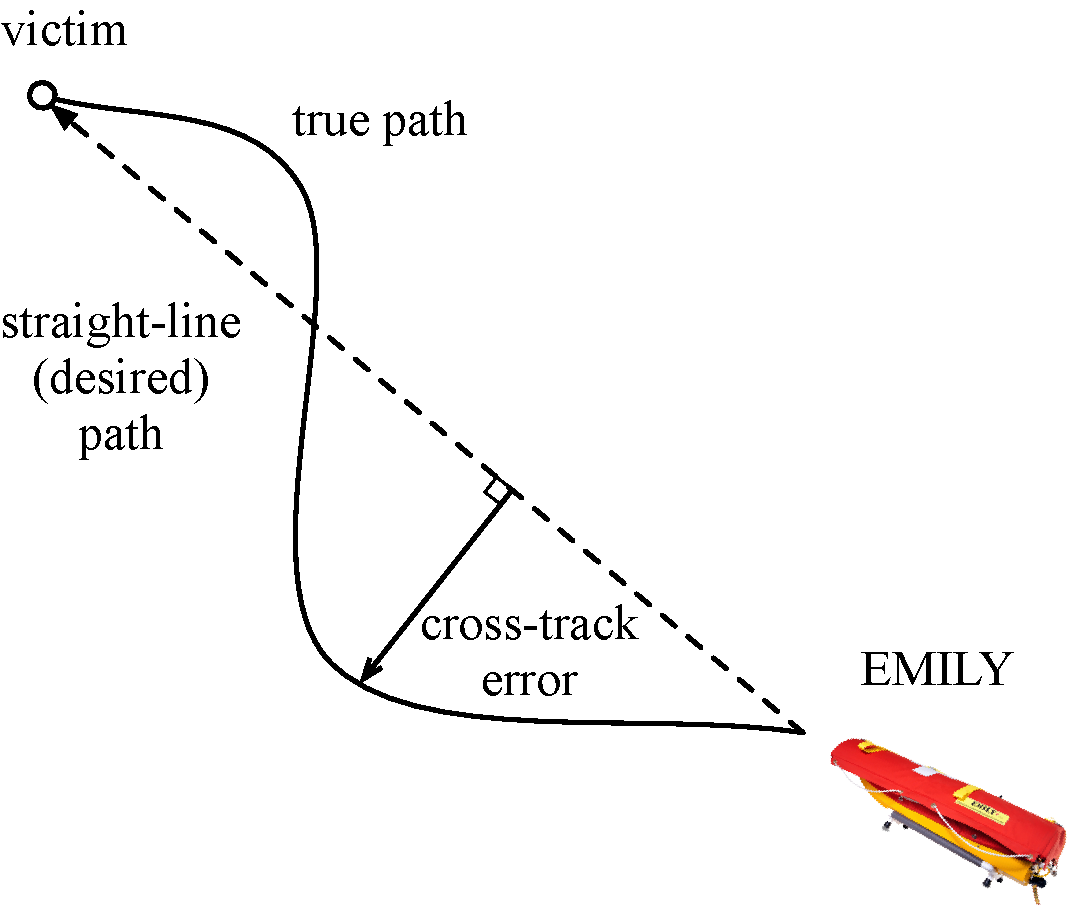
\includegraphics[scale=0.35]{figs/xte.pdf}
  \caption{Cross-track error}
  \label{fig:xte}
\end{figure}

The existing navigational system is organized in the following manner: a UAV vision system, developed by Dufek, \textit{et. al}, captures the craft's position and orientation, and transforms them to a global fixed frame \cite{dufek2016visual}. Then, an LOS geometric function determines the best reference heading for path-keeping with a straight path, and a proportional controller modifies the rudder position to achieve that heading reference, as detailed by Xiao, \textit{et. al} \cite{xiao2017uav}.  

Sec. \ref{sec:background} reviews the foundational literature on marine craft dynamics and control which are utilized in this project, as well as the relevant applications of learning-based controllers. Sec. \ref{sec:dynamic_model_and_simulation} discusses modeling the kinematics and dynamics of EMILY in a maritime rescue environment. Sec. \ref{sec:los} presents two line-of-sight geometric functions for determining the best heading reference for path-keeping, one of which is capable of supporting arbitrary parametric path functions, with some minor limitations. 

Inspired by the PID neural network controller found in marine literature, the team implemented a gradient descent-based tuning method for a standard PID controller, as detailed in Sec. \ref{sec:pid_neural_network}. Two sets of experiments are conducted: one to study tuning properties of the algorithm, and one to benchmark performance against the existing proportional (P) controller. The experimental design is discussed in Sec. \ref{sec:experimental_design}, with the results presented in Sec. \ref{sec:results_and_discussion}. The final sections present some concluding remarks, recommendations for further investigation, and practical considerations.

%%%%%%%%%%%%% BACKGROUND AND LIT REVIEW %%%%%%%%%%%
\section{Background and Literature Review}\label{sec:background}
Marine craft control has a rich and illustrious history in the broader control systems domain. All marine craft, EMILY included, experience several low-level challenges including: highly coupled and nonlinear dynamics, large degrees of freedom (DOF), and tendency of instability. In addition to these challenges, surface marine craft are often under-actuated and non-holonomic.

A proportional-integral-derivative (PID) controller is one of the oldest categories of linear feedback controller, and is used ubiquitously in industry. Incorporating an integral and derivative term allows the PID controller to react to error dynamics, typically improving tracking performance over the traditional P controller. In fact, the theoretical foundation for PID control was first developed by Minorsky for automatic ship steering systems \cite{minorsky1922directional}. For our purposes, employing an auto-tuned PID algorithm with resulting nonlinear dynamics rather than a nonlinear controller allows future collaborators to quickly understand the structure of the controller.
% and equip EMILY's controller with the functionality to adapt to new environments. \incomplete

Following the marine path-keeping literature, we decompose the navigation problem into finding the path and then keeping the path. For the latter component, Fossen presented line-of-sight (LOS) guidance for marine craft, which provides a geometric and parametric approach to finding the reference heading towards a desired path \cite{fossen2003line}. By adjusting the LOS radius, the path-keeping aggressiveness can be tuned. However, this parameter does have a profound effect on the resulting controller dynamics.

Artificial neural networks (ANN) and the backpropagation algorithm provide a computational approach to learning complex functional relationships \cite{rojas2013neural}. In the controls domain, several authors have begun utilizing ANNs to learn the black-box dynamics of a plant, or even in some situations, as the controller itself. In particular, Hernandez, \textit{et. al} published a neural network tuning algorithm for control of underwater autonomous vehicles (UAVs), however, the authors use a sigmoid function on the output layer, which somewhat arbitrarily constrains the PID gains to the interval from zero to one \cite{hernandez2016neural}. Most neural network-based controllers use a tracking error metric as the loss function, and attempt to approximate the gradient with respect to the weights, as exact computation of the gradient requires a model of the plant.

Following this pattern, a simple framework is provided by Huailin \cite{shu2000pid}, which employs P, I, and D type neurons, the latter two of which have first-order discrete dynamics, as a hidden layer in the network, and the reference value and measurement of the control signal as network inputs. Huailin also presents a method of approximating the gradient and backpropagating a cumulative tracking error loss function.


%%%%%%%%%%%%% NOMENCLATURE %%%%%%%%%%%%%%%%%%

% Acronyms A
\nomenclature[A]{LOS}{Line-of-Sight}
% \nomenclature[A]{ANN}{Artificial Neural Network}
\nomenclature[A]{EMILY}{EMergency Integrated Lifesaving lanYard}

% Terms T
\nomenclature[T]{surge}{longitudinal velocity in body frame}
\nomenclature[T]{yaw}{rotation about the azimuth axis}


% Kinematics K
\nomenclature[K]{$\bm{p}_b^n$}{vector to point $b$ (or origin of frame $\{b\}$) in frame $\{n\}$}
\nomenclature[K]{$\bm{p}_{ev}$}{vector from EMILY to victim (global frame)}
\nomenclature[K]{$\bm{v}_{nb}^n$}{translational velocity vector of frame $\{b\}$ w.r.t point $\{n\}$ in frame $\{n\}$}
\nomenclature[K]{$\bm{\omega}_{nb}^n$}{angular velocity vector of frame $\{b\}$ w.r.t frame $\{n\}$ in frame $\{n\}$}
\nomenclature[K]{$R_b^n$}{rotates a coordinate vector in frame $\{b\}$ to frame $\{n\}$}
\nomenclature[K]{$\reference$}{LOS reference heading}
\nomenclature[K]{$\measurement$}{measured value of heading ($= \theta$ above)}
\nomenclature[K]{$\error$}{error between reference and measured heading}

% Dynamics D
\nomenclature[D]{$u_1$}{Thrust control input, i.e., longitudinal velocity}
\nomenclature[D]{$u_2$}{Rudder angle control input, ($\phi$)}
\nomenclature[D]{$\alpha_i$}{generic lumped parameter for control plant (EMILY)}
\nomenclature[D]{$\zeta$}{longitudinal displacement variable}
\nomenclature[D]{$\theta$}{yaw (heading) angle}
% \nomenclature[V]{$u_2$}{Rudder angle control input, ($=\phi$)}
\nomenclature[V]{$E_{MCTE}$}{EMILY's mean cross-track error}
\nomenclature[V]{$e_{CTE}$}{EMILY's cross-track error at particular sample}
% \nomenclature[V]{$u_2$}{Rudder angle control input, ($=\phi$)}
% \nomenclature[V]{$u_2$}{Rudder angle control input, ($=\phi$)}


% Might replace these with more specific notation



\begin{framed}\label{nomenclature}
\printnomenclature
\end{framed}

%%%%%%%%%%%%%%%%%%%%%%%%%%%%%%%%%%%%%%%%%%%%%%

\section{Dynamic Model and Simulation} % (fold)
\label{sec:dynamic_model_and_simulation}

A simplified parametric dynamic model was developed in order to prototype controllers. Without explicit formulation of the controller dynamics, this model allows designers to quickly test whether a particular learning algorithm is capable of controlling a plant with similar dynamics to the EMILY platform. Physical parameters are estimated where necessary. All of the necessary code to reproduce the simulations is available online\footnote{\url{https://github.com/MitchAllain/gpid-csce635}}.

\subsection{Kinematics}
A detailed review of marine craft kinematic modeling conventions can be found in the 2002 book by Fossen \cite{fossen2011handbook}. In our implementation, we adopt two conventional frames: the  North-East-Down (global) coordinate frame and the body-fixed coordinate frame, which are denoted  $\{n\}$ and $\{b\}$, respectively. A  coordinate vector to a point  $a$ expressed in the frame $\{n\}$ is denoted $\bm{p}_a^n$. For example, $\bm{p}_e^n$ and $\bm{p}_v^n$ define the coordinate vector to EMILY and the victim in the inertial frame. These two frames are illustrated in Fig. \ref{fig:kin}.

The EMILY craft is non-holonomic, having only a rear rudder and longitudinal propulsion. For simplicity, only dynamics in the longitudinal (called surge) direction and yaw orientation are modeled here. \textit{In the absence of current}, EMILY's velocity is denoted as
\begin{equation}
  \bm{v}_{nb}^b = [\dot{\zeta}, 0, 0]^T
\end{equation}
where $\bm{v}_{nb}^b$ is the velocity of the body frame with respect to the global frame, expressed in the body frame, and $\dot{\zeta}$ is used to denote longitudinal velocity. The rotational velocity is expressed as
\begin{equation}
  \bm{\omega}_{nb}^b = [0, 0, \dot{\theta}]^T
\end{equation}
where $\bm{\omega}_{nb}^b$ is the angular velocity of the body frame with respect to the global frame, and $\theta$ denotes the yaw angle, or the angle between unit vectors $n_1$ and $b_1$. The rotation matrix $R_b^n$ relates a coordinate vector in frame $\{b\}$ to frame $\{n\}$ and is defined as
\begin{align}
  R_b^n &= 
  \begin{bmatrix}
    n_1 \cdot b_1   &   n_1 \cdot b_2   &   n_1 \cdot b_3 \\
    n_2 \cdot b_1   &   n_2 \cdot b_2   &   n_2 \cdot b_3 \\
    n_3 \cdot b_1   &   n_3 \cdot b_3   &   n_3 \cdot b_3
  \end{bmatrix} \nonumber \\ \nonumber \\
  &=
  \begin{bmatrix}
    cos(\theta)   &   -sin(\theta)  &   0 \\
    sin(\theta)   &   cos(\theta)   &   0 \\
    0   &   0   &   1
  \end{bmatrix}
\end{align}
% . In the body frame $\{b\}$, EMILY has a longitudinal velocity (called surge), denoted $\zeta$. The yaw orientation of the craft is defined as $\theta$, the angle between the body frame and the computer vision frame, which is assumed to be fixed frame. For simplicity, EMILY is fully defined here in her workspace with 3 degrees of freedom (DOF), which we denote $q = [x, y, \theta]$. This assumption neglects pitch, roll, and heave, which are mainly relevant to stability control on larger craft. These kinematic variables are illustrated in Fig. \incomplete.

\begin{figure}[h]
  \centering
  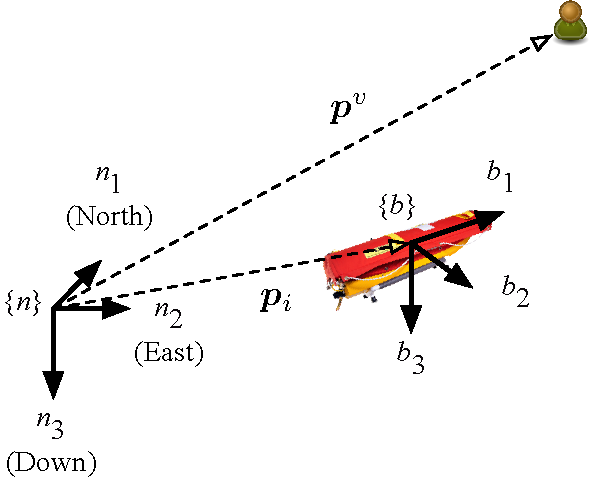
\includegraphics[scale=0.6]{figs/kin.pdf}
  \caption{Kinematic coordinate frames}
  \label{fig:kin}
\end{figure}

In simulation, the effect of irrotational currents is considered as a constant additive velocity perturbation in the global frame, $\bm{v}_c^n = [c_x, c_y]$, yielding total translation velocity
\begin{equation}
  \bm{v}_{nb}^n = R_b^n \bm{v}_{nb}^b + \bm{v}_c^n
\end{equation}
Therefore, the position of EMILY at time $t$ is given by
\begin{equation}
  \bm{p}_e^n(t) = \int_0^t (R_b^n \bm{v}_{nb}^b + \bm{v}_c^n)d\tau + \bm{p}_e^n(0)
\end{equation}
where $\bm{p}_e^n(0)$ is EMILY's initial position.

The orientation of EMILY at time $t$ is given by
\begin{equation}
  \Theta_{nb}(t) = \int_0^t \cancelto{I_{3 \times 3}}{T_b (\Theta_{nb})} \hspace{0.8cm} \bm{\omega}_{nb}^b d\tau + \Theta_{nb}(0)
\end{equation}
or simply,
\begin{equation}
  \theta(t) = \int_0^t \dot{\theta}d\tau + \theta(0)
\end{equation}
where $\theta(0)$ is EMILY's initial orientation in the global frame.
\subsection{Hydrodynamics}
The longitudinal equation of motion is given by:
\begin{equation}
  \ddot{\zeta} = \frac{1}{m}[u_1 - \alpha_1 \dot{\zeta}^2] 
\end{equation}
where $u_1$ is the thrust force due to the rear jet and $m$ is the mass of the craft. The lumped parameter $\alpha_1$ describes hydrodynamic drag force, defined by
\begin{equation}
  \alpha_1 = \frac{1}{2} C_D A_{fs} \rho
\end{equation}
where $C_D$ is the empirical drag coefficient and $A_{fs}$ is the frontal submerged surface area of the craft.

Assuming irrotational currents, yaw rotation is caused by a turning moment produced by the rear rudder. The rotational dynamics can be described with the following equation of motion:
\begin{equation}
  I \ddot{\theta} = \alpha_2 \cos(u_2) F_N - b \dot{\theta}
\end{equation}
where $I$ is the rotational inertia about the center of gravity, $\alpha_2$ is distance from the craft's center of gravity (COG) to the rudder axis. $F_N$ is the rudder drag force, and $u_2$ is the commanded angle for the rudder. Although the drag force does not act directly through the rudder axis, the distance has a minuscule effect on the resulting moment arm.

The drag force $F_n$ on the rudder is determined semi-empirically from \cite{zelazny2014approximate} using the following relation
\begin{equation}
   F_N = \frac{1}{2} \frac{6.13 \lambda}{\lambda + 2.25} A_r V_r^2 \rho
 \end{equation} 
Here, $\rho$ is the density of the fluid, $\lambda$ is the aspect ratio of the rudder, $A_r$ is the rudder area, and $V_r$ is the relative velocity of the fluid, i.e.,
\begin{equation}
  V_r = \dot{\zeta} - (\bm{v}_{c} \cdot \hat{b}_1)
\end{equation}
where $(\bm{v}_{c} \cdot \hat{b}_1)$ is the magnitude of the current in the longitudinal direction of the craft.

Combined, Eqs. (3-5) become:
\begin{equation}
  \ddot{\theta} = \alpha_2 \alpha_3 (\dot{\zeta} - (\bm{v}_{c} \cdot \hat{b}_1)^2 \cos(u_2) - \alpha_4 \dot{\theta}
\end{equation}
with lumped parameters:
\begin{align}
  \alpha_3 &= \left(\frac{1}{2I} \frac{6.13 \lambda}{\lambda + 2.25} A_r \rho \right) \\
  \alpha_4 &= \frac{b}{I}
\end{align}

See the Sec \ref{sec:states} in the appendix for the parameter values used in simulation and the listed state equations. 

% \subsection{Simulation}
% The system model was implemented using MATLAB and Simulink


% section dynamic_model_and_simulation (end)

\section{Line-of-Sight Algorithms}\label{sec:los}
Two line-of-sight (LOS) algorithms were developed simulataneously. The first is optimized for straight paths and utilizes the simplified geometry. The second LOS controller utilizes a multivariate unconstrained optimization approach to allow for generic reference paths, such as polynomial splines.

\textit{Note}: all proceeding coordinate vectors are expressed in the global (fixed) frame, $\{n\}$, and the superscripts will be omitted for convenience.

\subsection{Straight Path LOS} % (fold)
\label{sub:straight_path_los}

Given a straight reference path, the resulting LOS geometry is shown in Fig. \ref{fig:los}, where the point $i$ is EMILY's initial position, $e$ is EMILY's current position, $v$ is the victim, $a$ is the orthogonal intersection with the straight path, and $b$ is the LOS radius intersection with the path.
The coordinate vector to point a is computed as
\begin{equation}
  \bm{p}_a = \text{proj}_{\bm{p}_{ie}} \bm{p}_{iv} + \bm{p}_{i} = \frac{(\bm{p}_{ie} \cdot \bm{p}_{iv})}{||\bm{p}_{iv}||^2} \bm{p}_{iv} + \bm{p}_{i}
\end{equation}
which is used to define the vector to the intersection point $b$
\begin{equation}
  \bm{p}_{b} = \bm{p}_{a} + d_{ab} \frac{\bm{p}_{iv}}{||\bm{p}_{iv}||}
\end{equation}
where $d_{ab}$ is the distance between points $a$ and $b$
\begin{equation}
  d_{ab} = \sqrt{r^2 - \cte^2}
\end{equation}
Here, $r$ is the LOS radius parameter and $\cte$ is the computed cross-track error
\begin{equation}
  \cte = \frac{||\bm{p}_{ev} \times \bm{p}_{iv}||}{||\bm{p}_{iv}||}
\end{equation}
The coordinate vector from EMILY to the intersection point is
\begin{equation}
  \bm{p}_{eb} = \bm{p}_{b} - \bm{p}_{e}
\end{equation}
where the heading reference angle can be computed
\begin{equation}
  \reference = \text{atan2}(\bm{p}_{eb,y}, \bm{p}_{eb,x})
\end{equation}
Eqs. (17-22) are implemented in Algorithm \ref{alg:straight_los}.

\begin{algorithm}[h]
\caption{Straight path LOS heading}\label{alg:straight_los}
\begin{algorithmic}[1]
% \label{alg:pred}
\Function{Straight-LOS-Heading}{$\bm{p}_{e}, \bm{p}_{i}, \bm{p}_{v}, r$}
\State $\bm{p}_{ie} \gets (\bm{p}_{e} - \bm{p}_{i})$
\State $\bm{p}_{iv} \gets (\bm{p}_{v} - \bm{p}_{i})$
\State $\bm{p}_{ev} \gets (\bm{p}_{v} - \bm{p}_{e})$
\State $  \cte \gets \frac{||\bm{p}_{ev} \times \bm{p}_{iv}||}{||\bm{p}_{iv}||}$
\State $\bm{p}_{b} \gets \text{proj}_{\bm{p}_{ie}} \bm{p}_{iv} + \bm{p}_{i} + \frac{\bm{p}_{iv}}{||\bm{p}_{iv}||} \sqrt{r^2 - \cte^2}$
\State $\bm{p}_{eb} \gets \bm{p}_{b} - \bm{p}_{e}$
\State $\reference = \text{atan2}(\bm{p}_{eb,y}, \bm{p}_{eb,x})$ \Comment two argument arctangent
\State \Return{$\reference, \cte$}
\EndFunction
\end{algorithmic}
\end{algorithm}

\begin{figure}[h]
  \centering
  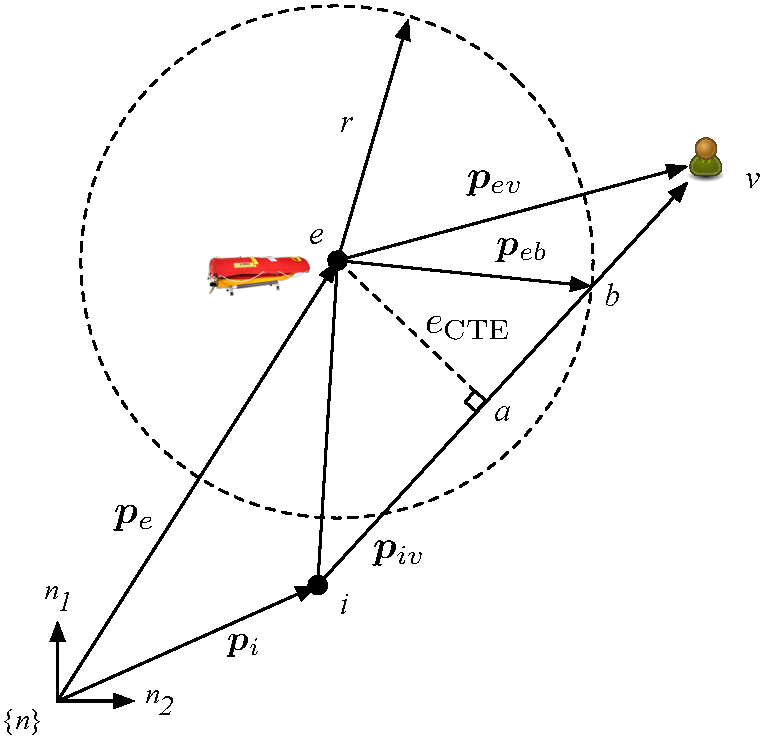
\includegraphics[scale=0.55]{figs/los.pdf}
  \caption{Straight path LOS geometry}
  \label{fig:los}
\end{figure}

% subsection straight_path_los (end)
\subsection{Parametric Path LOS} % (fold)
\label{sub:parametric_path_los}

The second LOS algorithm seeks to implement the same functionality with arbitrary parametric paths of type
\begin{equation}
  \bm{f}: s \mapsto [x, y]^T
\end{equation}
that is, the function maps a displacement parameter, $s$, to an $(x, y)$ coordinate in the global frame. For instance cubic splines could be generated from a selection of waypoints \cite{de1978practical}.

The approach utilizes a parametric representation of the LOS circle around EMILY
\begin{equation}
  \bm{p}_c(\psi) = \bm{p}_{e} + r \begin{bmatrix}
    \cos(\psi) \\ \sin(\psi)
  \end{bmatrix}
\end{equation}
where $\bm{p}_c(\psi)$ is the coordinate of a point on the circle at angle $\psi$. Then, we define a cost function
\begin{equation}
  J(\psi, s) = || \bm{f}(s) - \bm{p}_c(\psi) ||^2
\end{equation}
and run a multivariable minimization function such as MATLAB's \texttt{fminunc} (The MathWorks, Inc.), to result in the intersection parameters $[\psi^*, s^*]^T$, and intersection coordinates $\bm{p}_b = \bm{f}(s^*)$. Because there are typically two global minima (two intersections), the seeded parameter values for the search are the bearing to the victim and the point equal to the distance of one LOS radius projected straight forward from EMILY's position, and in the direction of EMILY's current heading. Still, the convergence properties of this approach are closely tied to the curvature of the path and the LOS radius parameter, and need to be studied more in depth.

\begin{algorithm}[h]
\caption{Arbitrary path LOS heading}\label{alg:arbitrary_los}
\begin{algorithmic}[1]
% \label{alg:pred}
\Function{F-Path-LOS-Heading}{$\bm{J}, \bm{p}_{e}, \bm{p}_{i}, \bm{p}_{v}, r$}
\State $\bm{p}_{ev} \gets (\bm{p}_{v} - \bm{p}_{e})$
\State $\bm{p}_{iv} \gets (\bm{p}_{v} - \bm{p}_{i})$
\State $s_0 \gets \bm{f}^{-1}(\bm{p}_{v})$ \Comment displacement at victim
\State $\psi_0 \gets \text{atan2}(\bm{p}_{ev,y}, \bm{p}_{ev,x})$ \Comment bearing to victim
\State $[s^*, \psi^*]^T \gets fminunc(J, [s_0, \psi_0])$
\State $\bm{p}_{b} \gets \bm{f}(s^*)$
\State $\bm{p}_{eb} \gets \bm{p}_{b} - \bm{p}_{e}$
\State $\reference = \text{atan2}(\bm{p}_{eb,y}, \bm{p}_{eb,x})$ \Comment two argument arctangent
\State \Return{$\reference$}
\EndFunction \\
\Function{Parametric-Circle, $\bm{p}_c$}{$\psi, \bm{p}_{e}, r$}
\State $\bm{p}_c \gets \bm{p}_{e} + r \begin{bmatrix} \cos(\psi) \\ \sin(\psi) \end{bmatrix}$
\State \Return{$\bm{p}_c$}
\EndFunction \\
\Function{Cost, $J$}{$\bm{f}, \bm{p}_c, s, \psi$}
\State $J \gets ||\bm{f}(s) - \bm{p}_c(\psi)||^2$
\State \Return{$J$}
\EndFunction
\end{algorithmic}
\end{algorithm}

% subsection parametric_path_los (end)

\section{Controller Design} % (fold)
\label{sec:pid_neural_network}
As discussed previously, the PIDNN presents a method of tuning PID gains in real-time. The network, as presented by Huailin, is illustrated in Fig. \ref{fig:pidnn}. The PIDNN network uses specialized P, I, and D type neurons with first-order discrete dynamics in the I and D neurons. The approach designates as a loss function the mean tracking error over a trailing window of samples, defined by
\begin{equation}
  J = \frac{1}{m} \sum\limits_{k=1}^{m} (r[k] - y[k])^2
\end{equation}
where $m$ is the window (memory) length, and $r[k]$ and $y[k]$ are the reference and measurement.

Although this is not equivalent to mean cross-track error, minimizing the mean tracking error results in better path keeping and reduced cross-track error. Further, backpropagating the cross-track error directly would require knowledge of the second (thrust) input and violate our design constraint. 

Taking the gradient with respect to each of the weights from the hidden layer to the output layer requires that input to system gradient be approximated as
\begin{equation}
  \frac{\partial y}{\partial u} \approx \frac{\Delta y}{\Delta u} = \frac{y[k] - y[k - 1]}{u[k] - u[k-1]}
\end{equation}
This approximation is the most significant limitation of the PIDNN approach, because it does not \textit{gaurantee} that the weight updates will move towards a lower tracking error.

The authors suspect that the published success of this controller was in part due to seeding weights on the first layer of the network such that the input to the hidden layer was exactly
\begin{equation}
  e = r - y
\end{equation}
i.e., the input layer weights are seeded at 1 and -1. Further in any heading controller, all orientation values must be wrapped at the interval from $[-\pi, \pi]$, i.e., for state $\theta$, each time step we enforce (using modular arithmetic)
\begin{align}
  \theta_{\text{wrap}} &= \theta + \pi \pmod{2\pi} \\
  \theta &= \theta_{\text{wrap}} - \pi
\end{align}
This modular heading computation is not possible within the original PIDNN framework. For these reasons, it is necessary to use a modified network architecture in our controller.

\begin{figure}[h]
\centering
\begin{subfigure}{.5\textwidth}
  \centering
  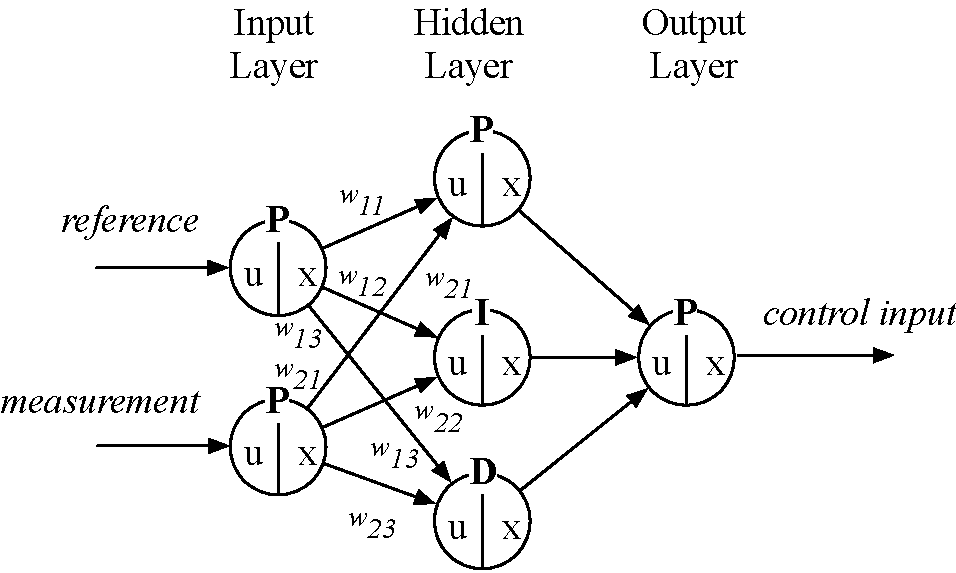
\includegraphics[width=0.8\linewidth]{figs/pidnn.pdf}
  \caption{PIDNN Controller \cite{shu2000pid}}
  \label{fig:pidnn}
\end{subfigure} \\ \vspace{0.5cm}
\begin{subfigure}{.5\textwidth}
  \centering
  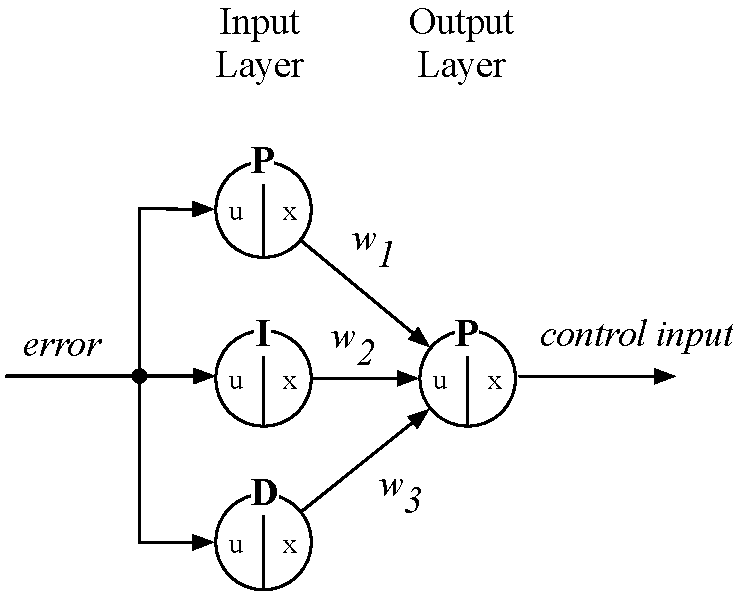
\includegraphics[width=.65\linewidth]{figs/gpid.pdf}
  \caption{GPID "network"}
  \label{fig:gpid}
\end{subfigure}
\caption{Comparison of PIDNN and GPID controllers}
\label{fig:controllers}
\end{figure}

\subsection{GPID Controller} % (fold)
\label{sub:gpid_controller}
By removing the input layer of the PIDNN, and replacing the inputs $\reference$ and $\measurement$ with the error, $\error$, we arrive at the network shown in Fig. \ref{fig:gpid}, which is, admittedly, more appropriately designated as a \textit{gradient-tuned PID (GPID)} on-line tuning algorithm. The loss function remains the same, as does the gradient with respect to the weights, which is
\begin{equation}
  \frac{\partial J}{\partial w_j} \approx -\frac{2}{m} \sum\limits_{k=1}^m e[k] \frac{y[k] - y[k - 1]}{u[k] - u[k-1]} x_j[k]
\end{equation}
The inside of the summation can be computed and stored at each time step to reduce computational cost, for which we will use the notation
\begin{equation}\label{eq:gradient}
  \frac{\partial J}{\partial w_j} \approx -\frac{2}{m} \sum\limits_{k=1}^m \delta_j[k] x_j[k]
\end{equation}
The resulting in update rule can be written as
\begin{equation}
  w_j[k + 1] = w_j[k] - \alpha_j \frac{\partial J}{\partial w_j}
\end{equation}
where $\alpha_j$ is an element of the learning rate vector. The pseudo-code for an update iteration of the GPID controller is shown in Algorithm \ref{alg:gpid_update}. The resulting navigational system is shown in Fig. \ref{fig:sys}.

\begin{figure*}[t]
  \centering
  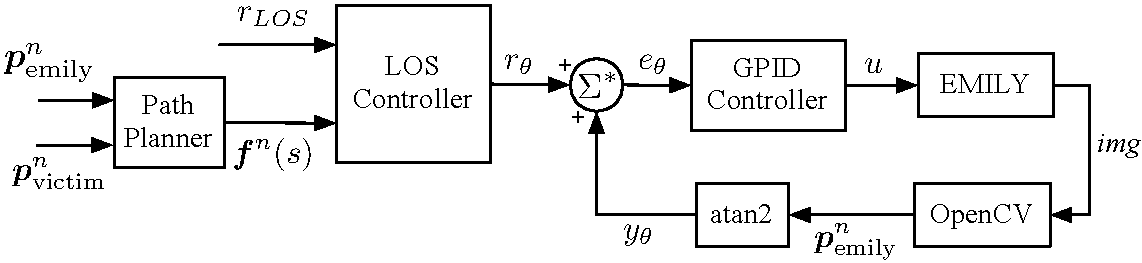
\includegraphics[scale=0.6]{figs/system_overview.pdf}
  \caption{The resulting navigational control system}
  \label{fig:sys}
\end{figure*}

\begin{algorithm}[h]
\caption{Update the GPID controller}\label{alg:gpid_update}
\begin{algorithmic}[1]
% \label{alg:pred}
\Function{Update-Controller}{$\error, \measurement, m$}
\State $u, x_1, x_2, x_3, x_4 \gets compute\_output(\error)$
\State push $\measurement$ to \textit{measurement\_mem} \Comment append to deque
\State push $\error$ to \textit{error\_mem}
\For{each neuron $i$}
\State push $x_i$ to \textit{output\_mem\_i}
\EndFor
\If{size of \textit{error\_mem} $> 1$}
\For{each weight $j$}
\State $\delta_j \gets$ Eq. \ref{eq:gradient} \Comment incremental gradient
\EndFor
\EndIf
\If{size of \textit{error\_mem} $== m$} \Comment if deque is full
\For{each weight $j$}
\State $\frac{\partial J}{\partial w_j} \gets \frac{-2}{m} \sum\limits_{k=1}^m  \delta_j[k] x_j[k]$ \Comment sum deque
\State $w_j \gets w_j - \alpha_j \frac{\partial J}{\partial w_j}$ \Comment backpropagate
\EndFor
\For{each queue}
\State pop oldest sample from queue
\EndFor
\EndIf
\State \Return{$u$}
\EndFunction
\end{algorithmic}
\end{algorithm}


% subsection gpid_controller (end)

% section pid_neural_network (end)

\newpage
\section{Experimental Design} % (fold)
\label{sec:experimental_design}
The objectives of experimentation were to 1) test the convergence properties of the GPID gains and 2) verify that the GPID controller is superior to the previously implemented proportional controller. Further, we sought to document any practical limitations of the controller, and simulate the integration in the navigation system as a whole.

\subsection{Simulation} % (fold)
\label{sub:simulation}
All tests were executed using a combination of Python scripts, MATLAB functions, and Simulink block diagrams. Two Simulink models were developed interfacing the kinematic and dynamic model of EMILY with the LOS and controller functions: one for the GPID controller and one with a traditional proportional controller. The Simulink models were fully parametric, such that both the physical parameters of EMILY and the test environment parameters could be defined at execution. The simulations were terminated once EMILY reached within a 10 meter radius of the victim\footnote{in implementation, the controller will switch to an entirely different scheme within a certain radius of the victim}. 

The output of each simulation includes two files, one with time series data for EMILY's position, measured heading, reference heading, the control input to the rudder, and the network weights if applicable, and one file with trial metadata such as path type, LOS radius, victim location, initial heading, ocean current velocity vector, throttle input value, network memory length, and network weight training rates.

The GPID controller itself was prototyped and tested in Python first for proof-of-concept. The calls to the network update function utilized MATLAB's ability to wrap Python objects and to convert the returned data to a MATLAB compatible data format.

% subsection simulation (end)

\subsection{GPID Tuning Properties}
The GPID algorithm is parameterized by a memory length and a vector of learning rates, both of which have a significant effect on the controller dynamics. To test the properties of the GPID controller over repeated trials, several simulations were run with the parameters drawn uniformly from the intervals in Table \ref{table:parameters}. EMILY began each trial at the origin of the global frame.

\begin{table}[h]
\normalsize
\centering
\begin{tabular}{c c c c}
% \hline
\rowcolor{gray!20}
Parameter & Description & Lower & Upper \\
\hline
$p_{v,x}$ & EMILY initial $x$ & -50 m & 50 m \\
$p_{v,y}$ & EMILY initial $y$ & -50 m & 50 m \\
$\theta_i$ & EMILY initial heading & $-\pi$ rad & $\pi$ rad \\
$c_x$ & current in $x$ direction & -0.66 m/s & 0.66 m/s \\
$c_y$ & current in $y$ direction & -0.66 m/s & 0.66 m/s \\
\hline
\\
\end{tabular}
\caption{Intervals for randomly selected parameters}\label{table:parameters}
\end{table}

\label{sec:results_and_discussion}
\begin{figure*}[h!]
  \centering
  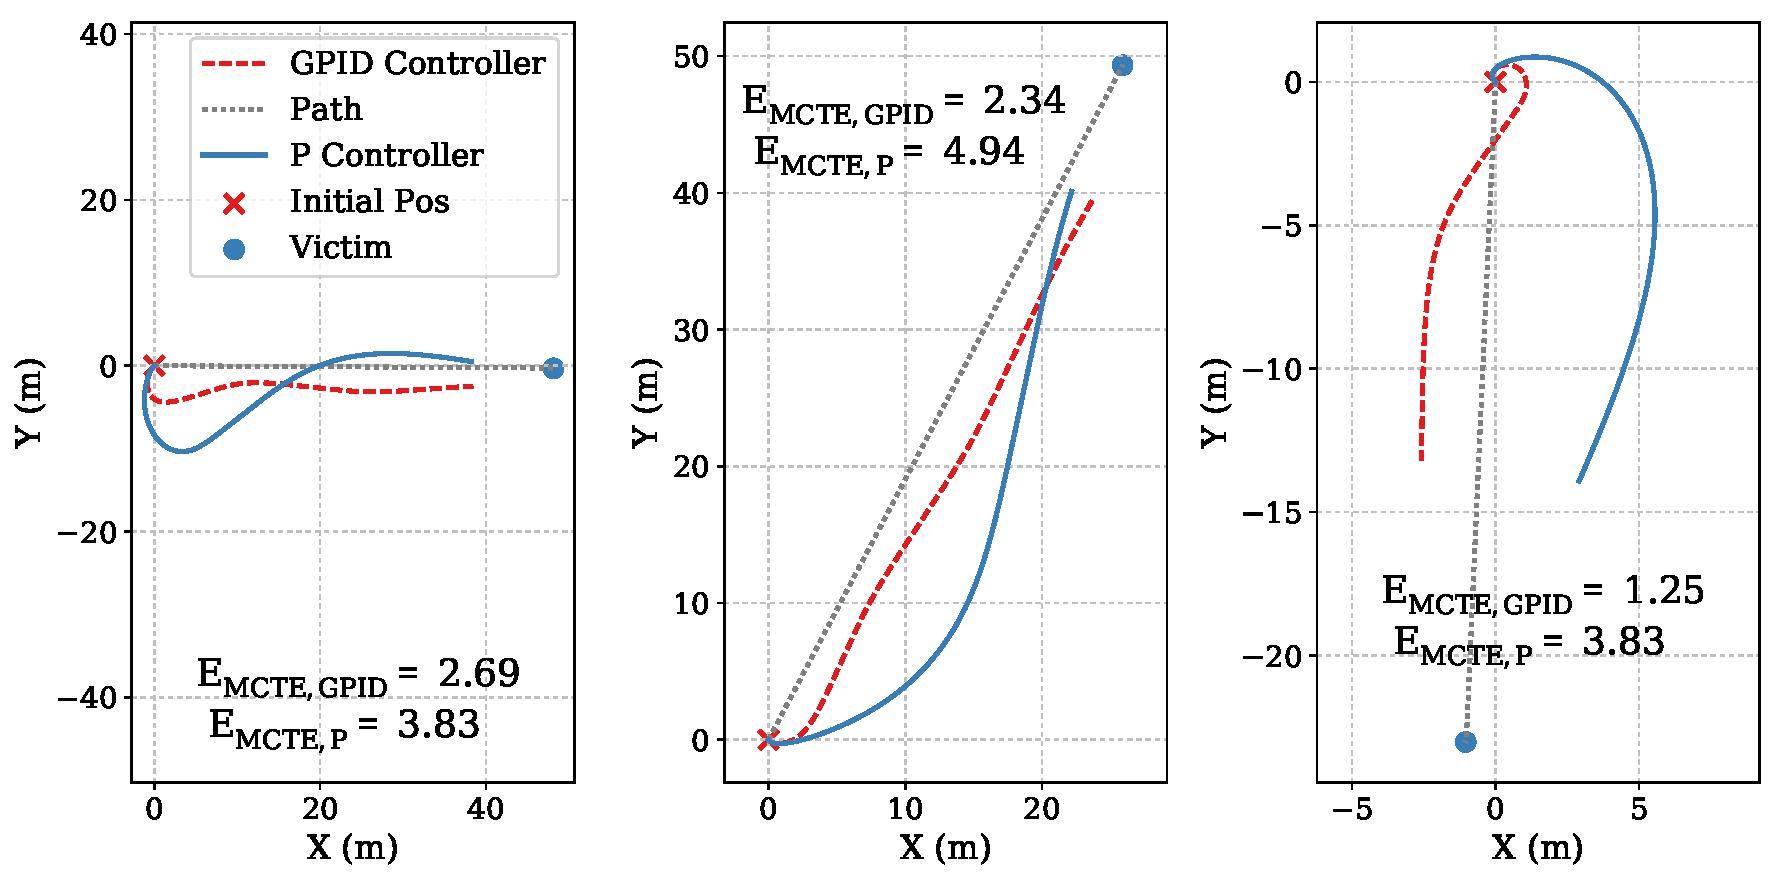
\includegraphics[scale=0.5]{figs/sample_trials.pdf}
  \caption{Three sample simulation results with the proportional and GPID controller. \textit{Note: the simulations terminate within a 10 m radius of the victim.}}
  \label{fig:sample}
\end{figure*}

\subsection{Performance Comparison}
In order to compare the two controllers in a structured way, a set of trials were planned holding all parameters constant except for one. In this manner, the robustness of each controller to variations in specific parameters could be studied. The parameters are:
\begin{itemize}
  \item the victim's position
  \item EMILY's initial heading
  \item the current direction and magnitude
  \item the throttle control input
  \item the path type
\end{itemize}
The values used in testing are displayed with the test results in the following section.
% section experimental_design (end)

\section{Results and Discussion} % (fold)


A significant number of iterations were required to converge on acceptable parameters for the GPID algorithm. Further, the tuning action will not stabilize an unstable system, so the weights (gains) must be initialized with values from a stable controller.

Once an operating range had been established for the network parameters, the team ran batches of trials with parameters in the neighborhood to test the sensitivity of the algorithm. The results of changes on memory length and learning rate on weight convergence and cross-track error are illustrated in Figs. \ref{fig:convergence} and  over the batch of trials. Since the cost function is constantly changing in response to the initial conditions and environmental dynamic of each trial, it is difficult to test for any properties of convergence. 

However, a memory too short can lead to oversensitivity to the transient conditions like poor initial heading or environmental disturbances. This effect is evident in the rapid changes of gains in Fig. \ref{fig:note_jumps}. On the contrary, large memory inhibits the controller's ability to respond to transient conditions (note the larger distribution on the second controller in Fig. \ref{fig:GPID_param}). A learning rate which is too aggressive can easily destabilize the system, however a learning too small tends to behave like a static PID system.

\begin{figure}[h]
\centering
\begin{subfigure}{.5\textwidth}
  \centering
  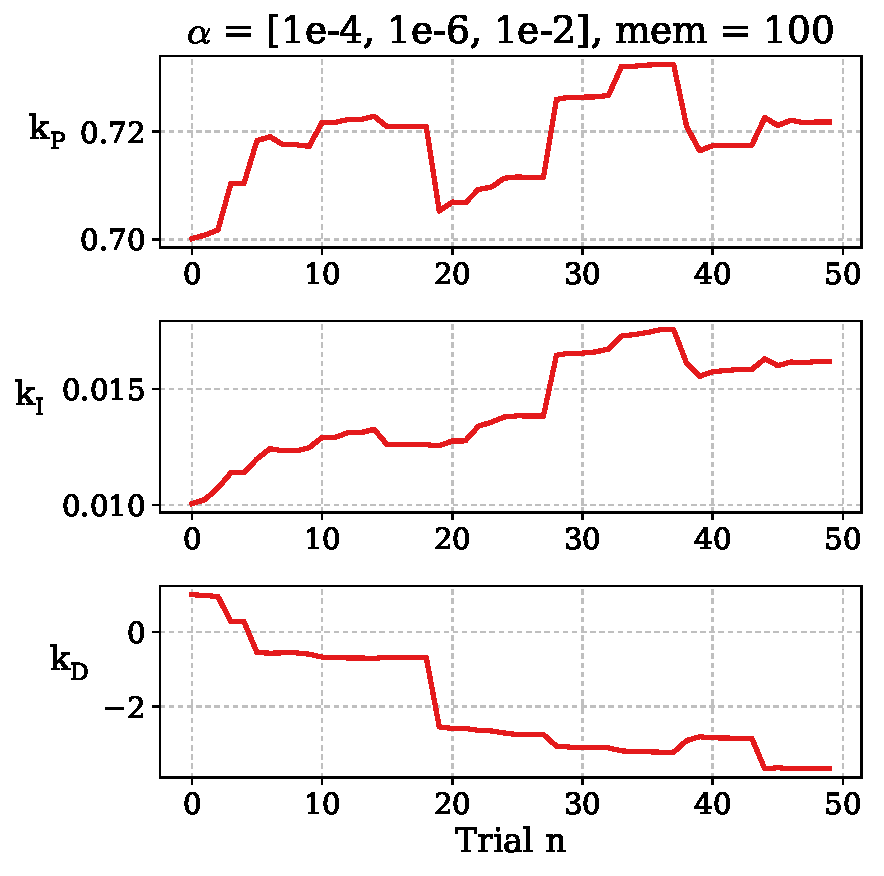
\includegraphics[width=0.7\linewidth]{figs/weight_05_07_t3.pdf}
  \caption{Short memory and low learning rate}
  \label{fig:note_jumps}
\end{subfigure} \\ \vspace{1cm}
\begin{subfigure}{.5\textwidth}
  \centering
  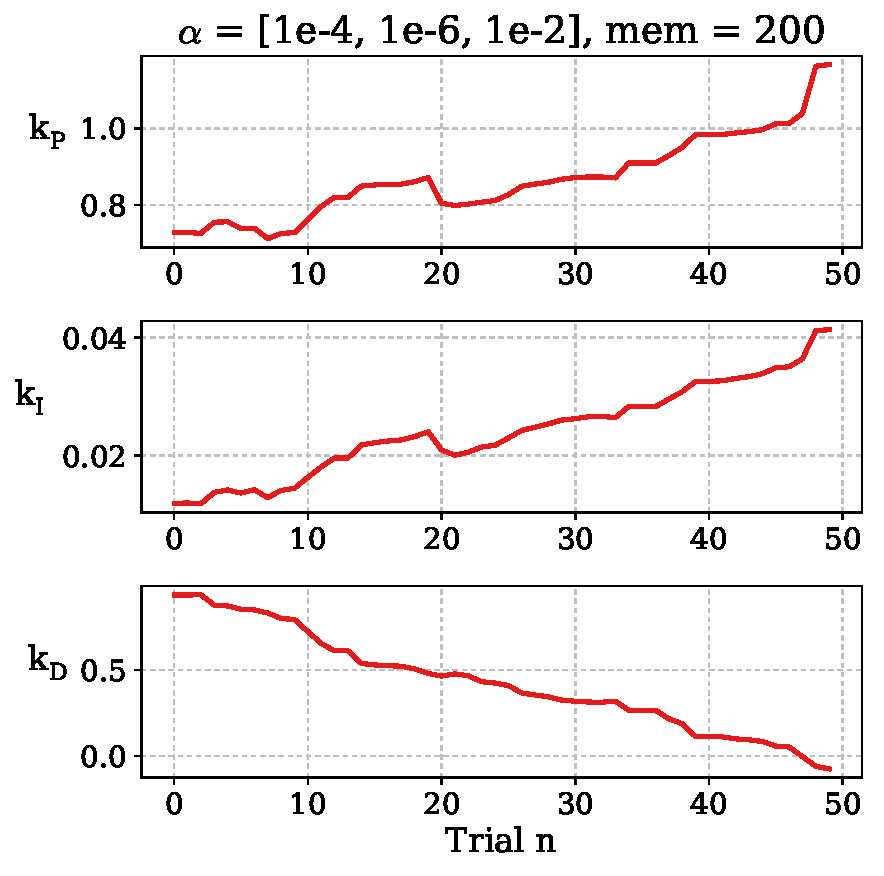
\includegraphics[width=.7\linewidth]{figs/weight_05_07_t5.pdf}
  \caption{Long memory and low learning rate}
\end{subfigure} \\ \vspace{1cm}
\begin{subfigure}{.5\textwidth}
  \centering
  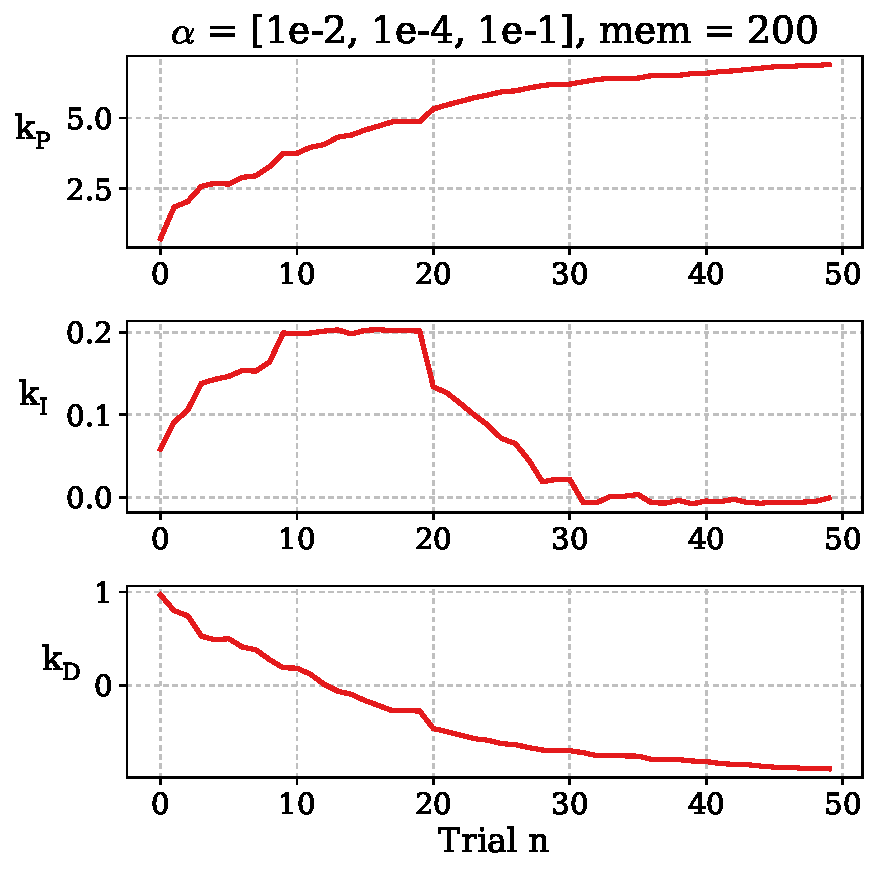
\includegraphics[width=.7\linewidth]{figs/weight_05_07_t6.pdf}
  \caption{Long memory and high learning rate}
\end{subfigure}
\caption{Effect of learning rate and memory on gain convergence}
\label{fig:convergence}
\end{figure}

\begin{figure}[h]
  \centering
  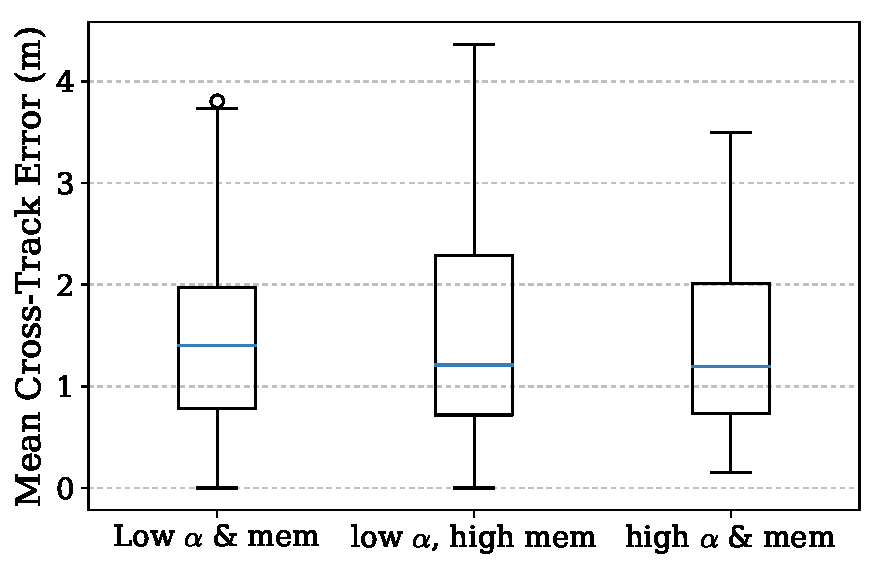
\includegraphics[scale=0.5]{figs/gpid_param.pdf}
  \caption{Mean cross-track error for the three GPID parameter sets, i.e., training rate vector $\alpha$ and memory, $m$}
  \label{fig:GPID_param}
\end{figure}

Sample trials for the GPID and proportional controllers are illustrated in Fig. \ref{fig:sample}, with mean cross-track error for both controllers inscribed in each subplot.

Structured trial parameters are displayed in Table \ref{table:str_trials}, along with the mean cross-track error for simulations with each controller. For each configuration (each row) all parameters were held constant \textit{except} for the parameter in the left hand column. Notable scenarios where the controller performance differed greatly include traveling against the current, traveling \textit{shorter} distances, and higher thrust values.

\begin{table}[h]\label{table:str_trials}
\normalsize
\centering
\begin{tabular}{c | c c c}
% \hline
\rowcolor{gray!20}
% Victim, $\bm{p}_v$ & Initial Heading, $\theta_i$ & Current, $\bm{v}_c$ & Throttle, $u_1$ & Path Type & P CTE & GPID CTE \\
% \hline
% [40, 40]^T  &   $180\deg$   &
Param & Values & P MCTE & GPID MCTE \\
\hline
& $180\degree$ & 4.248 & 0.980 \\
$\theta_i$ & $135\degree$ & 4.062 & 4.075 \\
& $225\degree$ & 4.075 & 0.705 \\
\hline \\
$\bm{p}_v$ & $[25, 25]^T$ & 5.439 & 1.142 \\
(m) & $[40, 40]^T$ & 4.248 & 0.980 \\
& $[100, 100]^T$ & 3.266 & 0.386 \\
\hline \\
& $[0, 0]^T$ & 4.248 & 0.980 \\
& $[0.3, 0.3]^T$ & 10.405 & 7.426 \\
$\bm{v}_c$ & $[-0.3, -0.3]^T$ & 3.616 & 0.366 \\
(m/s) & $[0.6, 0.6]^T$ & 5.955 & 1.507 \\
& $[-0.6, 0.6]^T$ & 45.437 & 39.405 \\
& $[-0.6, -0.6]^T$ & 8.055 & 0.524 \\
\hline \\
& \textit{straight} & 4.248 & 0.980 \\
Path & \textit{cubic 1} & 4.371 & 1.998 \\
Type & \textit{cubic 2} & 4.446 & 3.463 \\
& \textit{cubic 3} & 4.423 & 2.322 \\
\hline \\
thrust & 1.5 & 4.944 & 1.144 \\
(N) & 3 & 4.248 & 0.980 \\
& 6 & 3.573 & 0.409 \\
\hline
\hline
& \textbf{Average} & \textbf{7.754} & \textbf{4.162}
\end{tabular}
\caption{Varied parameters and effect on MCTE}\label{table:str_trials}
\end{table}


% section results_and_discussion (end)

\section{Conclusion}
The authors were tasked with improving and benchmarking a navigational control system for a  mobile marine buoy. Two line-of-sight geometric algorithms were presented which produce reference heading angles that converge to the desired path, either expressed as a straight line or a parametric curve. Then, a gradient-based proportional-integral-derivative (GPID) tuning method is discussed which utilizes a cumulative mean-squared-error cost function over a rotating memory and an approximate gradient descent to update the PID gain parameters in real-time. 

The results from all simulations lead our team to believe the GPID approach to tuning PID control parameters is significantly superior to the existing proportional controller. Algorithms for GPID and LOS control consistently produced lower cross-track error. The increased stability due to the GPID controller leads to shorter arrival times and more robustness to external perturbations. The gradient descent approximation gives EMILY the functionality to adapt to varying environments, form factors, and weight distributions. 

% conference papers do not normally have an appendix


% use section* for acknowledgment
\section*{Acknowledgment}
The authors would like to thank Dr. Murphy and her team of research assistants. A special thanks to Jan Dufek, who provided both insight and expertise throughout the development of this project. 


\section{Appendix}

\subsection{Recommendations}
The authors are confident that a PID-based control method is adequate for this system, although they suspect that the GPID controller, at its current level of development, may be too brittle for deployment. At a minimum, the weights should be saturated on an interval of known stable controllers. That way, a failed trial or the presence of a large disturbance could not completely disrupt the learning process, causing instability, rather the system would just degrade to a suboptimal, but stable, PID controller.


\subsection{State Equations}\label{sec:states}
The states variables and state equations are presented below in Table \ref{table:states} and Eqs (34-37). 
\begin{align}
% Position states
\dot{x}_1   &= x_2 \\
\dot{x}_2   &= \frac{1}{m}[u_1 - \alpha_1 x_2^2] \\
\dot{x}_3   &= x_4 \\
% Velocity States
\dot{x}_4   %&= \frac{1}{m_{1,rod}}(F_L + P_{1,A}A_{1,p,A}-P_{1,B}A_{1,p,B}) \\
      &= \alpha_2 \alpha_3 (x_2 - (\bm{v}_{c} \cdot \hat{b}_1))^2 \cos(u_2) - \alpha_4 x_4
\end{align}

\begin{table}[h!]\label{table:states}
\normalsize
\centering
\begin{tabular}{c l}
% \hline
\rowcolor{gray!20}
State & Description \\
\hline
%   & $\theta$    & Swing angular position \\
% 2  & $\dot{\theta}$ & Swing angular velocity \\
$x_1$  & Longitudinal displacement in body frame, $\zeta$ \\
$x_2$  & Longitudinal velocity in body frame, $\dot{\zeta}$\\
$x_3$  & Yaw angle, $\theta$ \\ 
$x_4$  & Yaw velocity, $\dot{\theta}$ \\
\hline
\\
\end{tabular}
\caption{Dynamic model states}\label{table:states}
\end{table}

\begin{table}[h!]
\normalsize
\centering
\begin{tabular}{L L L}
\rowcolor{gray!20}
\text{Parameter} & \text{Value} & \text{Units} \\
\hline
b           & 10       & Ns/m \\
m           & 40        & kg \\
C_D         & 0.6       & - \\
A_{fs}      & 0.03      & m^2 \\
\rho        & 1027      & kg/m^3 \\
\lambda     & 1.6    & - \\
A_r         & 0.015       & m^2 \\
I           & 7.5       & kg/m^2 \\
\\
\rowcolor{gray!20}
\text{Lumped Parameter} & \text{Value} & \text{Units} \\
\hline
\alpha_1         & 9.2       & kg/m \\
\alpha_2         & 0.5       & m \\
\alpha_3         & 2.31       & 1/m^3 \\
\alpha_4         & 1.33      & 1/s \\
% \beta
% \gamma
\end{tabular}
\caption{Simulation parameters, approximated for EMILY}\label{states}
\end{table}

\vspace{1in}

% trigger a \newpage just before the given reference
% number - used to balance the columns on the last page
% adjust value as needed - may need to be readjusted if
% the document is modified later
%\IEEEtriggeratref{8}
% The "triggered" command can be changed if desired:
%\IEEEtriggercmd{\enlargethispage{-5in}}

% references section

% can use a bibliography generated by BibTeX as a .bbl file
% BibTeX documentation can be easily obtained at:
% http://mirror.ctan.org/biblio/bibtex/contrib/doc/
% The IEEEtran BibTeX style support page is at:
% http://www.michaelshell.org/tex/ieeetran/bibtex/
\bibliographystyle{IEEEtran}
% argument is your BibTeX string definitions and bibliography database(s)
\bibliography{emily}
%
% <OR> manually copy in the resultant .bbl file
% set second argument of \begin to the number of references
% (used to reserve space for the reference number labels box)
% \begin{thebibliography}{1}

% \bibitem{IEEEhowto:kopka}
% H.~Kopka and P.~W. Daly, \emph{A Guide to \LaTeX}, 3rd~ed.\hskip 1em plus
%   0.5em minus 0.4em\relax Harlow, England: Addison-Wesley, 1999.

% \end{thebibliography}




% that's all folks
\end{document}


